\chapter{\ifproject%
\ifenglish Project Structure and Methodology\else โครงสร้างและขั้นตอนการทำงาน\fi
\else%
\ifenglish Project Structure\else โครงสร้างของโครงงาน\fi
\fi
}

% ในบทนี้จะกล่าวถึงหลักการ และการออกแบบระบบ

\makeatletter

% \renewcommand\section{\@startsection {section}{1}{\z@}%
%                                    {13.5ex \@plus -1ex \@minus -.2ex}%
%                                    {2.3ex \@plus.2ex}%
%                                    {\normalfont\large\bfseries}}

\makeatother
%\vspace{2ex}
% \titleformat{\section}{\normalfont\bfseries}{\thesection}{1em}{}
% \titlespacing*{\section}{0pt}{10ex}{0pt}

\section{Methodology}

\begin{figure}
\begin{center}
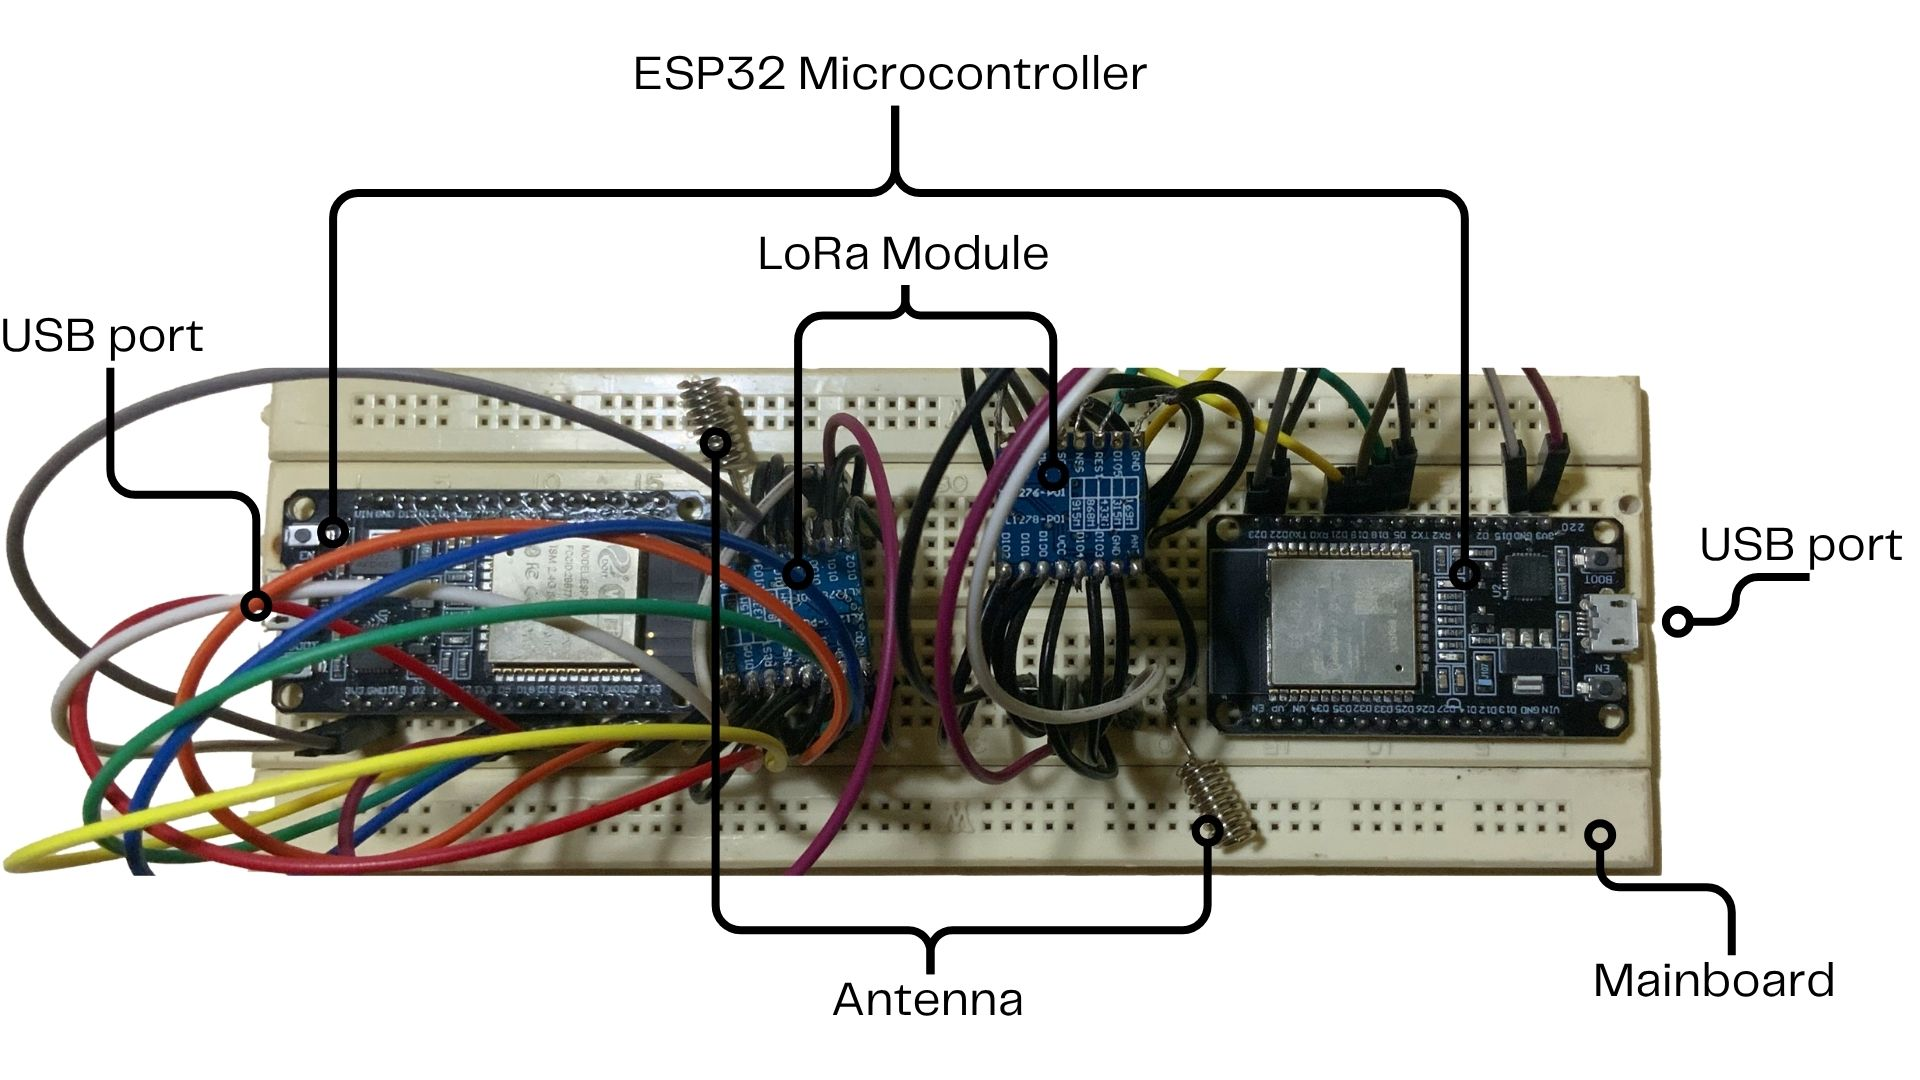
\includegraphics[width=0.8\textwidth]{Architecture.jpg}
\end{center}
\caption[Picture]{Design Architecture}
\label{fig:walrus}
\end{figure}

\subsection{System Architecture}
 The proposed framework consists of two ESP32 devices, each connected to a LoRa SX1276 module. One device operates as the sender (initiator), and the other as the receiver (responder). The devices communicate over LoRa to exchange verification and application messages. The overall architecture ensures that both devices can generate identical session keys without directly transmitting key material.

\subsection{RSSI-Based Key Generation}
To synchronize RSSI values, one device (the initiator) first transmits a known verification message. The receiving device measures the RSSI of this signal and attempts to decode the message using its reading. If decryption fails, the receiver iteratively adjusts its interpretation by shifting the RSSI value up or down within a pre-agreed tolerance interval (e.g., ±0.5 dBm) until the message is correctly decrypted. Unlike static pre-shared keys, which remain fixed and are vulnerable once compromised, session keys in this framework are dynamically derived from RSSI. Since RSSI is measured uniquely at the receiver and varies naturally with the environment, it is difficult for an attacker to predict or replicate. Security is further enhanced by concatenating the RSSI values and sampling them across multiple frequency channels into an array. 

\subsection{Keyword Verification}
To ensure correctness, both devices share a pre-defined keyword. After decryption, the receiver compares the result against this keyword. A match confirms that both devices are synchronized on the same session key. If the keyword is not matched, the process repeats until a valid session key is established.

\subsection{Implementation Details}
The framework is implemented on two ESP32 boards, each connected to LoRa SX1276 modules and powered via USB. Testing is carried out on prototype devices only, within a controlled laboratory environment. No end-user testing or real-world deployment is included.
The software stack consists of MicroPython firmware, Visual Studio Code, Thonny IDE, and the mpremote command-line tool. Simulated IoT messages are used as test data to evaluate the system. The variables measured include computation time, CPU usage, and memory consumption. 
